\documentclass[a4paper,11pt,twoside]{article}

\usepackage{amsmath}
\usepackage{amssymb}
\usepackage[english]{babel}
\usepackage{caption}
\usepackage{cite}
%\usepackage{cleveref}
\usepackage{color}
\usepackage{fancyhdr} % For the page headers
\usepackage{graphicx} % Including images
\usepackage{hyperref} % Including links
\usepackage{etoolbox}
\usepackage{longtable}
\usepackage{sectsty} % Makes changing \chapter, \section, etc. easier

\usepackage{catoptions}

\captionsetup{
  margin=10pt,
  font=small,
  labelfont=bf,
  position=top,
}

%% Math type specifying fonts
\newcommand{\V}[1]{\ensuremath{\mathbf{#1}}}
\newcommand{\s}[1]{\ensuremath{\mathcal{#1}}}

%% GA operators
\newcommand{\gp}{\ensuremath{\;}}
\newcommand{\gpi}{\ensuremath{\mathbin{/}}}
\newcommand{\lcont}{\ensuremath{\mathbin{\rfloor}}}
\newcommand{\rcont}{\ensuremath{\mathbin{\lfloor}}}
\newcommand{\dotp}{\ensuremath{\mathbin{\cdot}}}
\newcommand{\inverse}[1]{\ensuremath{#1^{-1}}}
\newcommand{\dual}[1]{\ensuremath{#1^\ast}}
\newcommand{\undual}[1]{\ensuremath{#1^{-\ast}}}
\newcommand{\edotp}{\ensuremath{\mathbin{\dotp_\mathbb{E}}}}
\newcommand{\elcont}{\ensuremath{\mathbin{\lcont_\mathbb{E}}}}
\newcommand{\ercont}{\ensuremath{\mathbin{\rcont_\mathbb{E}}}}
\newcommand{\edual}[1]{\ensuremath{#1 \lcont \inverse{\epseudo}}}
\newcommand{\eundual}[1]{\ensuremath{#1 \lcont \epseudo}}
%\newcommand{\edual}[1]{\ensuremath{#1^\bigstar}}
%\newcommand{\eundual}[1]{\ensuremath{#1^{-\bigstar}}}
\newcommand{\norm}[1]{\ensuremath{\left\|#1\right\|}}

\DeclareMathOperator{\pluckerid}{\Omega_q}
\DeclareMathOperator{\pluckerbilin}{\Omega}
\DeclareMathOperator{\Em}{Em}
\DeclareMathOperator{\grade}{\mathtt{grade}}
\newcommand{\pdual}[1]{\ensuremath{#1^\natural}}

\newcommand{\heq}{\ensuremath{\mathbin{=_{H}}}} % Homogeneous equality

%% Pl\"ucker notation
\newcommand{\plucker}[2]{\ensuremath{\{#1 \mathbin{:} #2\}}}
%\newcommand{\pluckerpoint}[2]{\ensuremath{(#1 \mathbin{:} #2)}}
%\newcommand{\pluckerplane}[2]{\ensuremath{[#1 \mathbin{:} #2]}}

%% Math-like symbols
\newcommand{\reals}{\ensuremath{\mathbb{R}}}
\newcommand{\en}{\ensuremath{\mathbin{\mbox{and}}}}
\newcommand{\of}{\ensuremath{\mathbin{\mbox{or}}}}
\newcommand{\eql}{\ensuremath{\Leftrightarrow}}

%% Math constants and shorthands
\newcommand{\pline}{\ensuremath{\ell}}
\newcommand{\rline}{\ensuremath{\ell_o}}
\newcommand{\iline}{\ensuremath{\ell_\infty}}
\newcommand{\screw}{\ensuremath{s}}

\newcommand{\ez}{\ensuremath{e_0}}
\newcommand{\ee}{\ensuremath{\V{e}_1}}
\newcommand{\et}{\ensuremath{\V{e}_2}}
\newcommand{\ed}{\ensuremath{\V{e}_3}}
\newcommand{\eze}{\ensuremath{e_{01}}}
\newcommand{\ezt}{\ensuremath{e_{02}}}
\newcommand{\ezd}{\ensuremath{e_{03}}}
\newcommand{\etd}{\ensuremath{e_{23}}}
\newcommand{\ede}{\ensuremath{e_{31}}}
\newcommand{\eet}{\ensuremath{e_{12}}}
\newcommand{\epseudo}{\ensuremath{\V{I}_3}}
\newcommand{\hpseudo}{\ensuremath{\ez\V{I}_3}}

\newcommand{\ap}{\ensuremath{a_{+}}}
\newcommand{\am}{\ensuremath{a_{-}}}
\newcommand{\bp}{\ensuremath{b_{+}}}
\newcommand{\bm}{\ensuremath{b_{-}}}
\newcommand{\cp}{\ensuremath{c_{+}}}
\newcommand{\cm}{\ensuremath{c_{-}}}

%% Text symbols
\newcommand{\newterm}{$^\dagger$}

\newcommand{\ega}{\texttt{e3ga}}
\newcommand{\pga}{\texttt{p3ga}}
\newcommand{\cga}{\texttt{c3ga}}
\newcommand{\cbga}{\texttt{c5ga}}
\newcommand{\iga}{\texttt{i2ga}}
\newcommand{\lga}{\texttt{l3ga}}

%% Setting color definitions
\definecolor{nicered}{rgb}{0.6, 0, 0.24}
\definecolor{nicegreen}{rgb}{0.0, 0.5, 0.24}
\definecolor{niceblue}{rgb}{0, 0.4, 1}
\definecolor{gray}{rgb}{0.2, 0.2, 0.2}
\definecolor{lightgray}{rgb}{0.4, 0.4, 0.4}

\newtoggle{draft}

\AtEndPreamble{
  \iftoggle{draft}{
    \hypersetup{
      colorlinks=true, 
      urlcolor=nicegreen,
      linkcolor=niceblue,
      citecolor=nicered,
    }
    \newcommand{\comment}[1]{\colorbox{red}{\bfseries\color{white}#1}}
    \newcommand{\TODO}[1]{\colorbox{niceblue}{\bfseries\color{white}TODO: #1}}
    \newcommand{\askLeo}[1]{\colorbox{yellow}{\bfseries Leo: #1}}
  }{
    \hypersetup{
      colorlinks=true,
      urlcolor=gray,
      linkcolor=gray,
      citecolor=lightgray,}
    \newcommand{\comment}[1]{}
    \newcommand{\TODO}[1]{}
    \newcommand{\askLeo}[1]{}
    }}

\makeatletter
%% Provide \Autoref; the \autoref with a printed capital
\def\figureautorefname{figure}
\def\tableautorefname{table}
\def\partautorefname{part}
\def\appendixautorefname{appendix}
\def\equationautorefname{equation}
\def\AMSautorefname{equation}
\def\theoremautorefname{theorem}
\def\Autoref#1{%
  \begingroup
  \edef\reserved@a{\cpttrimspaces{#1}}%
  \ifcsndefTF{r@#1}{%
    \xaftercsname{\expandafter\testreftype\@fourthoffive}
      {r@\reserved@a}.\\{#1}%
  }{%
    \ref{#1}%
  }%
  \endgroup
}
\def\testreftype#1.#2\\#3{%
  \ifcsndefTF{#1autorefname}{%
    \def\reserved@a##1##2\@nil{%
      \uppercase{\def\ref@name{##1}}%
      \csn@edef{#1autorefname}{\ref@name##2}%
      \autoref{#3}%
    }%
    \reserved@a#1\@nil
  }{%
    \autoref{#3}%
  }%
}

%% Commands for the title page.
% The title page needs the following data to be shown correctly:
% - \title
% - \subtitle (optional)
% - \studentid
% - \ects
% - \programme
% - \programmeaddress
% - \supervisor
% - \supervisoraddress
% - \finaldate or \date
\def\title#1{\gdef\@title{#1}}
\def\subtitle#1{\gdef\@subtitle{#1}}
\def\studentid#1{\gdef\@studentid{#1}}
\def\ects#1{\gdef\@ects{#1}}
\def\programme#1{\gdef\@programme{#1}}
\def\programmeaddress#1{\gdef\@programmeaddress{#1}}
\def\supervisor#1{\gdef\@supervisor{#1}}
\def\supervisoraddress#1{\gdef\@supervisoraddress{#1}}
\def\finaldate#1{\gdef\@finaldate{#1}}

\renewcommand{\maketitle}{
\begin{titlepage}
\begin{center}

\vspace{2.5cm}

\begin{Huge}
\@title
\end{Huge}
\rule{\linewidth}{0.1pt}

\ifdef{\@subtitle}{
\begin{large}
\@subtitle
\end{large}}{}

\vspace{1.5cm}

\@author\\
\@studentid

\vspace{1.5cm}

% [DO NOT CHANGE]
Bachelor thesis\\
% [CHANGE] Whether your Bachelor thesis is 6 ECTS (regular) or 9 ECTS (Honours
% programme).
Credits: \@ects{}EC

\vspace{0.5cm}

% [DO NOT CHANGE] The name of the educational programme.
\@programme

\vspace{0.25cm}

% [DO NOT CHANGE] The addess of the educational programme.
\@programmeaddress

\vspace{4cm}

\emph{Supervisor}\\
% [CHANGE] The name of your supervisor. Include the titles of your supervisor,
% as well as the initials for *all* of his/her first names.
\@supervisor

\vspace{0.25cm}

% [CHANGE] The address of the institute at which your supervisor is working.
% Be sure to include (1) institute (is appropriate), (2) faculty (if
% appropriate), (3) organisation name, (4) organisation address (2 lines).
\@supervisoraddress

\vspace{1.5cm}

% [CHANGE] The date at which you will finalize and submit your thesis.
\ifdef{\@finaldate}{\@finaldate}{\@date}

\end{center}
\addtocounter{page}{-1}
\end{titlepage}

}
\makeatother


\toggletrue{draft}

\title{Visualization of the projective line geometry for geometric algebra} % FIXME betere titel
\subtitle{Drawing lines in GAViewer}
\author{\href{mailto:dhrdekok@gmail.com}{Patrick de Kok}}
\studentid{5640318}
\ects{18}
\programme{Bacheloropleiding Kunstmatige Intelligentie}
\programmeaddress{University of Amsterdam\\Faculty of Science\\Science Park 904\\1098 XH Amsterdam}
\supervisor{\href{mailto:L.Dorst@uva.nl}{Dr.ir.\ Leo Dorst}}
\supervisoraddress{Intelligent Systems Laboratory Amsterdam\\Faculty of Science\\Science Park 904\\1098 XH Amsterdam}
\date{July 24th, 2012}

%%% Adding own commands, renew old ones
%\renewcommand{\familydefault}{\sfdefault}

\begin{document}
%\frontmatter
\iftoggle{draft}{
  \begin{center}
    \begin{Huge}
      {\color{red} NOTE!}
    \end{Huge}
  \end{center}
  This document contains some notes. Explanation of the notes:
  \begin{itemize}
    \item \colorbox{red}{\bfseries\color{white}Red comments}: directed to the reader in general.  These include questions like how to cite, how something could be rephrased, and questions on spelling.
    \item \colorbox{yellow}{\bfseries Yellow notes}: directed at the supervisor (\makeatletter\@supervisor\makeatother) which are on the subject of the thesis.
    \item \colorbox{niceblue}{\bfseries\color{white}Blue todos}: directed mostly at myself, but might be convenient for the general reader as well.
  \end{itemize}

Now let's start off with a question to the reader:

\comment{If putting a reference at the end of a sentence, how should that be done?}
\begin{enumerate}
  \item This is a reference to some article.~\cite{TheBook}
  \item This is a reference to some article~\cite{TheBook}.
\end{enumerate}

And a small caution:

\TODO{Fix table placement.}

    \setcounter{page}{-1}
  \newpage
}{}

\maketitle
\begin{abstract}
This thesis describes a method for computationally recognizing the geometrical interpretation of most blades of the model of projective line geometry in geometric algebra.  These different interpretations are not merely recognizable by the grade of the elements, or the absence or presence of some basis vector, as can be done for the homogeneous model for geometric algebra.  GAViewer, a graphical calculator for the Euclidean and conformal models of geometric algebra, is extended to implement the projective line geometry and its visualization.

\textbf{Keywords:} Geometric algebra, projective geometry, Pl\"ucker coordinates, homogeneous representation.

\end{abstract}
\tableofcontents

%\mainmatter
\section{Introduction}
\label{ch:introduction}

\comment{Needs to be written. Will be done in the end.}

\TODO{Cite \cite{Hongbo}, \cite[Chapter 2 and 3]{Pottmann}, \cite{Barrau1, Barrau2}}

%Just as linear algebra, geometric algebra is an algebra over a given vector space $\reals^n$.  The difference lies in its operations; whereas linear algebra relies on matrix manipulations which cannot always be inverted, geometric algebra's base operation is the geometric product.  From this invertible product, one can deduce the inner product, known from linear algebra, and the outer product.  The outer product grants the user access to the exterior algebra $\bigwedge \reals^n$.  The outer product of $\V{A}, \V{B} \in \bigwedge \reals^n: \V{A} \wedge \V{B}$ represents the set of elements that are linear combinations of its operands $\left\{\alpha \V{A} + \beta \V{B} \mid \alpha, \beta \in \reals \right\}$
%
%There are already several models of geometry in use in the geometric algebra community, of which the conformal model is the most popular and widely known~\cite{TheBook}.  Although usable in many cases, the transformations of the conformal model are a subset of those of the projective model. The projective transformations are an important class of operations within computer vision and computer graphics. 
%
%GAViewer is a visualization and computing tool for the 3-dimensional Euclidean and conformal models of geometric algebra, developed by Daniel Fontijne at the University of Amsterdam~\cite{GAViewer}.  It allows the user to perform calculations in geometric algebra, and shows the results, both numerical as well as graphical.  Moreover, it allows the user to rotate, translate and zoom the viewport, as well as to manipulate the displayed elements.  The variables in which they are stored are automatically updated, and, if desired by the user, other objects that are parameterized by the manipulated object, may be updated dynamically as well.
%
%Recently, Li and Zhang~\cite{Hongbo} have found a way to model projective geometry, using a 6 dimensional representation space $\reals^{3,3}$ with a special metric, which allows three basis vectors to square to $-1$.  Using Pl\"ucker coordinates~(\cite{Hongbo},\cite[Chapter 2]{Pottmann}), lines in 3-dimensional Euclidean space $\mathbb{E}^3$ are represented in the representation space by vectors $\V{v}^2 = \V{v} \V{v} = \V{v} \cdot \V{v} = 0$.  As a consequence, there are also vectors in the representation space $\V{w}^2 \not= 0$ which do not represent lines in $\mathbb{E}^3$.  Different geometrical objects are generated by the outer product over lines and non-lines.  For example, for two intersecting lines $\ell_1, \ell_2$, the outer product $\ell_1 \wedge \ell_2$ represents a pencil, the collection of all lines that are in the same plane as $\ell_1$ and $\ell_2$, and pass through the same point.  Taking the outer product of this pencil with a third intersecting line that does not lie in the same plane, results in a bundle; the set of all lines intersecting in a certain point.  This could be used to represent points in our space of lines.
%
%In their article, Li and Zhang have not discussed what each element in their algebra might represent.  Barrau~\cite{Barrau1,Barrau2} and Pottmann and Wallner~\cite[Chapter 2 and 3]{Pottmann} have investigated the objects that can be represented in a 6-dimensional space with Pl\"ucker coordinates, both using a different algebra from ours.  Pottmann and Wallner use linear algebra, while Barrau's algebra has less expressive power.  


\subsection{Project aim and document structure}
\TODO{Needs work.  Don't talk about project aim, but research question.}

\comment{I quote this from the first line of the introduction.  Put ``quotes'' around?} 
GAViewer is a multi-purpose program for performing geometric algebra computations and visualizing geometric algebra~\cite{GAViewer}.  The aim of this project is to augment GAViewer so it can interpret the Pl\"ucker model for geometric algebra.  Besides knowing how to evaluate textual expressions to objects of the algebra, GAViewer needs new interpretation and visualization algorithms.

In \autoref{ch:background}, a short introduction to geometric algebra and the Pl\"ucker model for linear algebra are given.  The algebra and model are coupled by interpreting the inner product with the help of the homogeneous model.  \Autoref{ch:research} demonstrates the geometric interpretation of several blades of the Pl\"ucker model.  The computation of characteristics needed to draw certain blades together with their sensible visualization are described in \autoref{ch:implementation}.

This document concludes at \autoref{ch:conclusion} with a discussion of this work as well as possible future work, and a bibliography.

\section{Projective geometry and geometric algebra}
\label{ch:background}

Geometric algebra is a mathematical framework for expressing geometric problems in a structure-preserving way.  This means that, in a well-defined model, applying an operation on a composed object of the algebra results in the same object as when one decomposes the object, applying the same operation on its decomposition, and compose the new object from the transformed elements.  Models that have this property, are called operational.

The system of Pl\"ucker coordinates is another framework for geometric problems; more specifically, projective line geometry.  It is often used with linear algebra and computer graphics~\cite{Shoemake}, and there have been non-operational models based on the homogeneous model in geometric algebra~\cite[Chapter 12]{TheBook}.  Recently, an operational model has been designed~\cite{Hongbo}.

\Autoref{sec:intro-ga} presents a short introduction to geometric algebra, while the operational model of Pl\"ucker coordinates for geometric algebra is explained in \autoref{sec:plucker}.

\subsection{Geometric algebra}
\label{sec:intro-ga}
\comment{Paraphrase Moos Hueting's work?  Nah, I can do better.}

\comment{Include the next notation explanation:}
\begin{itemize}
  \item Bold for Euclidean
  \item Capital for multivectors
  \item Lowercase for vectors/1-blades
  \item Greek for scalars/0-blades
  \item $\reals^{3,3}$
  \item Geometric product: $A \gp B$ $\leftarrow$ small space
  \item Geometric division $A \gpi B$ or too trivial?
  \item Outer product $\wedge$
  \item Left contraction $\lcont$
  \item Dot product $\dotp$
  \item Dualization $\dual{A}$, undualization $\undual{A}$
  \item Euclidean (un-)dualization $\edual{\V{A}}$, $\eundual{\V{A}}$ or introduce extra notation $\V{A}^{\star}$, $\V{A}^{-\star}$?
  %\item Euclidean inproduct $\elcont$? $A \edotp B$, $A \elcont B$, $A \ercont B$\ldots
  \item \ldots
  \item Show that geometric product, cross product can be expressed in terms of $\wedge$ and $\lcont$ for $\Em$.
\end{itemize}

\subsection{Pl\"ucker model}
\label{sec:hongbo}
\label{sec:plucker}
\comment{This part will be paraphrased from \cite{TheBook} and \cite{Hongbo}.  Where do I put the ref to \cite{TheBook}?}

\comment{Are all weighted lines directed lines?}

Weighted, infinitely-extending lines of $\reals^3$ have 5 degrees of freedom.  Such a line can be fully described by five numeric quantities. First, take a vector $\V{p}$ to a point on the line.  The point should be chosen so that the vector is orthogonal to the line.  The direction and weight of the line is given by a vector $\V{d}$.  These vectors are denoted in \autoref{fig:linedef}.

\begin{figure}
  \caption{A weighted line $L$ can be defined by any two of its weighted direction $\V{d}$, a vector $\V{p}$ orthogonal to the line, and its moment $\V{m} = \V{p} \times \V{d}$.}
  \label{fig:linedef}
  \begin{center}
    \fbox{
      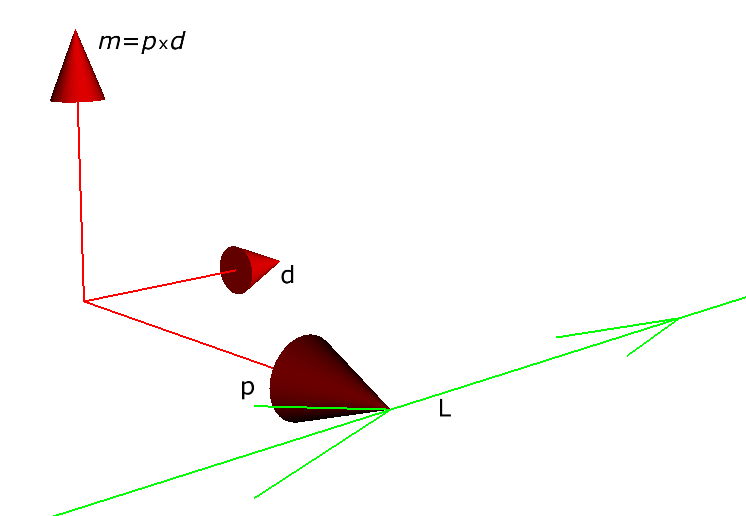
\includegraphics[width=0.6\textwidth]{linedef}
    }
  \end{center}
\end{figure}

In the homogeneous model, the line through points $p = \ez + \V{p}$ and $q = \ez + \V{q}$ is represented as 
\begin{equation*}
  L = p \wedge q = \ez \wedge (\V{q} - \V{p}) + \V{p} \wedge \V{q} ,
\end{equation*}
with the following dependency relationship: 
\begin{equation} \label{eq:gaplucker0} 
  \ez \wedge (\V{q} - \V{p}) \wedge (\V{p} \wedge \V{q}) = 0 .
\end{equation}

This relationship limits the number of degrees of freedom from 6 to 5.

The direction and moment of a line are easily recognised in this expression.  The direction $\V{d} = \V{p} - \V{q}$ is encoded in the first factor as $\ez \wedge -\V{d} = \V{d} \wedge \ez = \V{d} \ez$.  
The moment $\V{m} = \V{p} \times \V{q} = \edual{(\V{p} \wedge \V{q})}$ can be found in the second term as $\eundual{\V{m}} = \eundual{(\edual{(\V{p} \wedge \V{q})})} = \V{p} \wedge \V{q}$, which results in another general formula for lines:
\begin{equation*}
  L = \V{d} \ez + \eundual{\V{m}}.
\end{equation*}

Within classical literature of linear algebra, the same object is written as $-\plucker{\V{d}}{\V{m}}$, using \emph{Pl\"ucker coordinates} to denote a line as a 6D vector.  The constraint of \autoref{eq:gaplucker0} is expressed as 
\begin{equation} \label{eq:laplucker0}
  \V{d} \dotp \V{m} = 0 .
\end{equation}

The set of 6D vectors $-\plucker{\V{d}}{\V{m}}$ that comply with this constraint correspond to the points on the Klein quadric.

The Pl\"ucker coordinates of a line are often treated as just six slots for storing numbers.  In most cases, operations on these elements are defined to manipulate two 3D vectors, \V{d} and \V{m}, instead of the whole 6D element.

Because of this, the user is often unaware of most of the algebraic structure.  In fact, this 6D vector corresponds to
\begin{equation*}
  L = d_1 \ez\ee + d_2 \ez\et + d_3 \ez\ed + m_1 \et\ed + m_2 \ed\ee + m_3 \ee\et .
\end{equation*}

The set $\{\ez\ee, \ez\et, \ez\ed, \et\ed, \ed\ee, \ee\et\}$ forms an orthogonal and complete basis of the bivectors of the homogeneous model of $\reals^3$.  It is orthogonal, because for any two elements $x, y$ it holds that $x \lcont y = 0$. It is also complete; it contains $(^4_2) = 6$ linear independent elements.

The Pl\"ucker model uses these six elements as its basis; it treats these bivectors as 1-dimensional elements.  These elements will be known as $\{\eze, \ezt, \ezd, \etd, \ede, \eet\}$.  Li and Zhang~\cite{Hongbo} define an embedding from the Pl\"ucker model to the homogeneous model:
\begin{equation} \label{eq:Em}
  \Em(x) = \left\{ 
    \begin{array}{ll}
      \ez \wedge \V{e}_i &\mbox{if $x = e_{0i}$}; \\
      \V{e}_i \wedge \V{e}_j &\mbox{if $x = e_{ij}$}; \\
      \Em(y) + \Em(z) &\mbox{if $x = y + z$}; \\
      \Em(y) \wedge \Em(z) &\mbox{if $x = y \wedge z$}; \\
      \left[\Em(y) \wedge \Em(z)\right] &\mbox{if $x = y \lcont z$}. \\
    \end{array}
    \right.
\end{equation}

In the last line, the inner product for the Pl\"ucker is defined.  The bracket returns the proportionality factor of $\Em(y) \wedge \Em(z)$ to the homogeneous pseudoscalar $\hpseudo$.  This metric gives the multiplication table of \autoref{tab:nullmetric}.  Li and Zhang show that lines correspond with the null vectors of this space.  Because each of its basis elements correspond to a null vector, this basis is called the null basis. 

\begin{table}
  \caption{The multiplication table of the inner product for the Pl\"ucker model on the null basis.}
  \label{tab:nullmetric}
  \begin{center}
    \begin{tabular}{|c||c|c|c|c|c|c|}
      \hline
      $\lcont$ & $\eze$ & $\ezt$ & $\ezt$ & $\etd$ & $\ede$ & $\eet$ \\
      \hline \hline
      $\eze$ & 0 & 0 & 0 & 1 & 0 & 0 \\
      \hline
      $\ezt$ & 0 & 0 & 0 & 0 & 1 & 0 \\
      \hline
      $\ezd$ & 0 & 0 & 0 & 0 & 0 & 1 \\
      \hline
      $\etd$ & 1 & 0 & 0 & 0 & 0 & 0 \\
      \hline
      $\ede$ & 0 & 1 & 0 & 0 & 0 & 0 \\
      \hline
      $\eet$ & 0 & 0 & 1 & 0 & 0 & 0 \\
      \hline
    \end{tabular}
  \end{center}
\end{table}

Li and Zhang also show that the 6D space has the metric structure of $\reals^{3,3}$.  To demonstrate this structure, a second basis is given:

\begin{equation*}
  \begin{split}
  \left\{\ap, \bp, \cp, \am, \bm, \cm\right\} =
    & \left\{ \frac{\eze + \etd}{\sqrt{2}}, \frac{\ezt + \ede}{\sqrt{2}}, \frac{\ezd + \eet}{\sqrt{2}}, \right.\\
    & \left.  \frac{\eze - \etd}{\sqrt{2}}, \frac{\ezt - \ede}{\sqrt{2}}, \frac{\ezd - \eet}{\sqrt{2}}, \right\}
.
\end{split}
\end{equation*}

Without changing the semantics of the inner product, we obtain the multiplication table of \autoref{tab:screwmetric}.  It is apparent that the metric structure is $\reals^{3,3}$; three basis vectors, $\ap, \bp, \cp$, square to $1$, while the other three basis vectors, $\am, \bm, \cm$ square to $-1$.  

\begin{table}
  \caption{The multiplication table of the inner product for the Pl\"ucker model on the screw basis.}
  \label{tab:screwmetric}
  \begin{center}
    \begin{tabular}{|c||c|c|c|c|c|c|}
      \hline
      $\lcont$ & $\ap$ & $\bp$ & $\cp$ & $\am$ & $\bm$ & $\cm$ \\
      \hline \hline
      $\ap$ & 1 & 0 & 0 & 0 & 0 & 0 \\
      \hline
      $\bp$ & 0 & 1 & 0 & 0 & 0 & 0 \\
      \hline
      $\cp$ & 0 & 0 & 1 & 0 & 0 & 0 \\
      \hline
      $\am$ & 0 & 0 & 0 & -1 & 0 & 0 \\
      \hline
      $\bm$ & 0 & 0 & 0 & 0 & -1 & 0 \\
      \hline
      $\cm$ & 0 & 0 & 0 & 0 & 0 & -1 \\
      \hline
    \end{tabular}
  \end{center}
\end{table}

It is also clear that the basis elements do not represent lines, as no basis vectors squares to $0$.  \Autoref{ch:research} demonstrates that all non-null vectors of the Pl\"ucker model represent screw axes.  

This screw basis is good to demonstrate the metric structure of the model.  However, the null basis makes the connection to the homogeneous model more transparant.  

\subsubsection{Intersecting lines}
The classical approach of linear algebra~\cite{Shoemake} gives a formula to test if two lines $L_1 = -\plucker{\V{d}_1}{\V{m}_1}, L_2 = -\plucker{\V{d}_2}{\V{m}_2}$ coplanar: $\V{d}_1 \dotp \V{m}_2 + \V{d}_2 \dotp \V{m}_1 = 0$.  This expression can be translated to our model:

\begin{align*}
  0 &= \V{d}_1 \dotp \V{m}_2 + \V{d}_2 \dotp \V{m}_1 \\
    &= \left( d_{1,1} m_{2,1} + d_{1,2} m_{2,2} + d_{1,3} m_{2,3} \right) + \left( d_{2,1} m_{1,1} + d_{2,2} m_{1,2} + d_{2,3} m_{1,3} \right) \\
    &= d_{1,1} m_{2,1} + d_{1,2} m_{2,2} + d_{1,3} m_{2,3} + m_{1,1} d_{2,1} + m_{1,2} d_{2,2} + m_{1,3} d_{2,3} \\
    &= d_{1,1} \eze \lcont m_{2,1} \etd + d_{1,2} \ezt \lcont m_{2,2} \ede + d_{1,3} \ezd \lcont m_{2,3} \eet \\
    &\quad + m_{1,1} \etd \lcont d_{2,1} \eze + m_{1,2} \ede \lcont d_{2,2} \ezt + m_{1,3} \eet \lcont d_{2,3} \ezd \\
    &= \Em^{-1}\left( \V{d}_1\ez + \eundual{\V{m}_1} \right) \lcont \Em^{-1}\left( \V{d}_2\ez + \eundual{\V{m}_2} \right) \\
    &= \ell_1 \lcont \ell_2,
\end{align*}

with $\ell_1, \ell_2$ the null vectors of the Pl\"ucker model corresponding to $L_1, L_2$.  This test for coplanarity is a projective interpretation of intersection.  Points at infinity are not any different from other points.  Because of this property, one can say they intersect in the point at infinity.  This test for intersection also gives a geometric interpretation to the inner product of the Pl\"ucker model.

To test for intersection in a finite point, or to test for parallel lines, are tests that are not based on projective qualities.  Even though, a coordinate based version is given for both tests~\cite{Shoemake}.

To find the homogeneous point of intersection, one should solve the equation:
\begin{align*}
  \V{m}_1 \times \V{d}_1 + t \V{d}_1 + \V{d}_1^2 \ez &= \V{m}_2 \times \V{d}_2 + t \V{d}_2 + \V{d}_2^2 \ez &\longleftrightarrow \\
  t &= \frac{\V{m}_1 \times \V{d}_1 + \V{d}_2 \times \V{m}_2 + (\V{d}_1^2 - \V{d}_2^2) \ez}{\V{d}_2 - \V{d}_1} \\
  &= \frac{\eundual{\left( \V{m}_1 \V{d}_1 + \V{d}_2 \V{m}_2 \right)} + \left( \V{d}_1^2 - \V{d}_2^2 \right) \ez} {\V{d}_2 - \V{d}_1}
\end{align*}

Testing if lines $L_1$ and $L_2$ are parallel can be done by: 
\begin{align*}
  0 &= \V{d}_1 \times \V{d}_2 \\
    &= \left( \V{d}_1 \V{d}_2 \right) \lcont \epseudo
\end{align*}

\comment{Or should I just drop the last two formul\ae?}

\section{Classifying and parameterizing elements of different geometric interpretations}
\label{ch:research}

Before an implementation of a visualization can be made for a model, the geometric aspects of the elements of the model must be investigated.  A full inventory of the geometric elements has been done~\cite[Chapter 3]{Pottmann}, but in different terms.  Those terms are traditional, but do not hint at the geometric concept.  Besides the traditional terms, geometric inspired terms will be used.  

The following sections will discuss all geometrically different blades of a certain grade, together with their duals.  Besides text, each part has an accompanying table that contains the following information on the discussed blades:
\begin{itemize}
  \item \texttt{g}: the grade of the blade.
  \item $B^2$: the square of the blade, if it is a scalar value.  It could be either greater than, equal to, less than or not equal to 0, respectively indicated with $> 0$, $= 0$, $< 0$ and $\not= 0$.
  \item $B^2$: the square of the blade.  The relation of this scalar value to zero is indicated in the table with $> 0$, $= 0$, $< 0$ and $\not= 0$.
  \item Form: the general formula.  A blade factor can be either a line or screw axis, denoted by $\pline$ and $\screw$.  In certain cases, the difference between a real and ideal line is made with $\rline$ and $\iline$.  Here it does not concern any algebraic difference.  The difference is based on the visualization.  In other cases, a small textual note is given to indicate that the factors coincide at a single point (``pt.\ int.'') or in a plane (``pl.\ int.''), intersect each other pairwise (``pw.\ int''), or no factors intersect at all (``skew'').
  \item Visualization: the picture of a typical blade of this type.
  \item Name: what the blade class is named.  Traditional names, if needed, have been referenced.  In case of non-geometrically inspired terms, a more geometric alternative is given.  These are marked with ``\newterm''.
\end{itemize}

\TODO{Add pictures!}

\subsection{Elements of grade 0 and 6}
\begin{table}
  \caption{An inventory of the blades of grade 0 and 6.}
  \label{tab:inv0}
  \begin{center}
    \begin{tabular}{|c|r|l|c|l|}
      \hline
      \multicolumn{1}{|c|}{\texttt{g}} & $B^2$ & \multicolumn{1}{|c|}{Form} & \multicolumn{1}{|c|}{Graphical representation} & \multicolumn{1}{|c|}{Name} \\ \hline
      \hline
      0 & $\in \reals$ & $1 = \dual{I_6}$ & & Scalar~\cite{TheBook} \\ \hline
      6 & $\in \reals$ & $I_6 = \dual{1}$ & & Pseudoscalar~\cite{TheBook} \\ \hline
    \end{tabular}
  \end{center}
\end{table}

Scalars and pseudoscalars are interpreted the same as in other models for geometric algebra.  Scalars can be used to represent angles, weights, and many other scalar quantities.  Its dual, the pseudoscalar, may be utilized to denote the subspace volume, as well as for dualization.

\askLeo{Explain a bit more about pseudoscalar? Or scrap this whole section?}

\subsection{Elements of grade 1 and 5}
\begin{table}
  \caption{An inventory of the blades of grade 1 and 5.  
    \askLeo{Should I distinguish $\rline$ and $\iline$ in these tables?}}
  \label{tab:inv1}
  \begin{center}
    \begin{tabular}{|c|r|p{2.7cm}|p{2cm}|p{5cm}|}
      \hline
      \multicolumn{1}{|c|}{\texttt{g}} & $B^2$ & \multicolumn{1}{|c|}{Form} & \multicolumn{1}{|c|}{Visualization} & \multicolumn{1}{|c|}{Name} \\ \hline
      \hline
      1 & $= 0$ & $\rline$ & & Real line, path normal for uniform rotating motion\\ \hline
      1 & $= 0$ & $\iline$ & & Ideal line, path normal for uniform translating motion\\ \hline
      1 & $\not= 0$ & $\screw$ & & Screw axis \\ \hline
      5 & $= 0$ & $\dual{\rline}$ & & Singular linear complex~\cite{Pottmann}, uniform rotating motion \\ \hline
      5 & $= 0$ & $\dual{\iline}$ & & Singular linear complex~\cite{Pottmann}, uniform translating motion \\ \hline
      5 & $\not= 0$ & $\dual{\screw}$ & & Regular linear complex~\cite{Pottmann}, screw motion \\ \hline
    \end{tabular}
  \end{center}
\end{table}

It is clear from \autoref{sec:plucker} that the null vectors of the Pl\"ucker model (those vectors $v$ satisfying the Pl\"ucker identity $\pluckerid(v) = 0$) are interpreted as lines.  Let $l = d_1 \eze + d_2 \ezt + d_3 \ezd + m_1 \etd + m_2 \ede + m_3 \eet$ be a null vector.  The line can be interpreted through the homogeneous model.  The direction of the line corresponds to $\Em(d_1 \eze + d_2 \ezt + d_3 \ezd) \lcont -\ez = (d_1 \ee + d_2 \et + d_3 \ed)$, while its moment is $\V{m} = \edual{\Em(m_1 \etd + m_2 \ede + m_3 \eet)} = m_1 \ee + m_2 \et + m_3 \ed$.

Ideal lines cannot be interpreted in this way.  The homogeneous model treats these purely Euclidean elements as bivectors.  In the Pl\"ucker model, there is no such thing as a purely Euclidean element, which leaves room for interpretation in a projective way.  These elements represent lines at infinity, or ideal lines.  One can visualize an ideal line $l_\infty = \beta_1 \etd + \beta_2 \ede + \beta_3 \eet$ as a horizon, a circle on the heavenly sphere in direction $\Em(l_\infty)$.  

The vectors that do not square to $0$ can be interpreted as the dual of a helical, or screw motion~\cite[Section 3.1.2]{Pottmann}.  A screw motion simultaneously translates and rotates an object.  The object is translated along the same line as around which the rotation is performed.  The motion can be fully characterized by this line $a$ and the pitch $p$, the amount of translation per rotation.  For the grade 5 screw motion $S = \dual{\plucker{\V{d}}{\V{m}}}$, its pitch and axis are given by ~\cite[Theorem 3.1.9]{Pottmann}:
\begin{align}
  \label{eq:screwparams}
  p &= \V{d} \lcont \V{m} / \V{d}^2 \nonumber \\
  a &= \plucker{\V{d}}{\V{m} - p \V{d}} .
\end{align}

From this, one can deduce what kind of objects the dual elements of real and ideal lines represent.  For an ideal line $l_\infty$ with $p = 0 \lcont \V{m} / 0^2 = \infty$ and $a = \plucker{0}{\V{m} - \infty 0} = l_\infty$, we see that it is a pure translation; even the slightest bit of rotation lets the object be translated.  Given a real line $l_o$, its pitch is $p = 0 / \V{d}^2 = 0$, because of the Pl\"ucker identity, seen in \autoref{eq:laplucker0}.  Its axis is $a = \plucker{\V{d}}{\V{m} - 0} = l_o$.  No matter how much of the rotation is applied, no translation will occur.  This shows that the real lines are the duals of pure rotational motions.

These results are presented summarized in \autoref{tab:inv1}. 


\subsection{Elements of grade 2 and 4}
\begin{table}
  \caption{An inventory of the blades of grade 2 and 4.}
  \label{tab:inv2}
  \begin{center}
    \begin{tabular}{|c|r|p{2.7cm}|p{2cm}|p{5cm}|}
      \hline
      \multicolumn{1}{|c|}{\texttt{g}} & $B^2$ & \multicolumn{1}{|c|}{Form} & \multicolumn{1}{|c|}{Graphical representation} & \multicolumn{1}{|c|}{Name} \\ \hline
      \hline
      2 & $= 0$ & $\pline \wedge \pline$, pt.\ int. & & Pencil of linear line complexes~\cite{Pottmann}, pencil of lines~\cite{Hongbo} \\ \hline
      2 & $> 0$ & $\pline \wedge \pline$, skew & & Hyperbolic pencil of linear complexes~\cite{Pottmann}, Skew line pair~\newterm \\ \hline
      2 & $\not= 0$ & $\pline \wedge \screw$ & \comment{HIDE THIS ROW} & Parabolic pencil of linear complexes~\cite{Pottmann} \\ \hline
      2 & $< 0$ & $\screw \wedge \screw$ & \comment{HIDE THIS ROW} & Elliptic pencil of linear complexes~\cite{Pottmann} \\ \hline
      4 & $= 0$ & $\dual{\left( \pline \wedge \pline \right)}$ & & Pencil of singular linear complexes~\cite{Pottmann}, dual pencil of lines \\ \hline
      4 & $> 0$ & $\dual{\left( \pline \wedge \pline \right)}$, skew & & Hyperbolic linear congruence~\cite{Pottmann}, dual skew line pair~\newterm \\ \hline
      4 & $\not= 0$ & $\dual{\left( \pline \wedge \screw \right)}$ & \comment{HIDE THIS ROW} & Parabolic linear congruence~\cite{Pottmann} \\ \hline
      4 & $< 0$ & $\dual{\left( \screw \wedge \screw \right)}$ & \comment{HIDE THIS ROW} & Elliptic linear congruence~\cite{Pottmann}, pencil of reguli~\newterm \\ \hline
    \end{tabular}
  \end{center}
\end{table}

A two-blade $C = a \wedge b$ represents the set of linear combinations of $a$ and $b$:
\begin{equation*}
  \s{C} = \left\{ c \mid c \wedge C = 0 \right\} = \left\{ \lambda a + \mu b \mid \lambda, \mu \in \reals \right\} .
\end{equation*}
For the geometric interpretation of these blades, clarity on what kind of objects are in this set is needed.  On first inspection, this can be split in three cases, based on the number of null vectors among the factors.  We will limit this discussion to the case where both $a$ and $b$ are null vectors.

\comment{Easy way out. I don't understand Pottmann enough on this.}

\TODO{Two screws}

\TODO{Line and screw}

A linear combination $c = \lambda a + \mu b$ is a null vector if:
\begin{align}
  \label{eq:lincombnull}
  c^2 &= (\lambda a + \mu b) \lcont (\lambda a + \mu b) \nonumber \\
  &= \lambda^2 a^2 + 2 \lambda \mu a \lcont b + \mu^2 b^2 \nonumber \\
  &= 2 \lambda \mu a \lcont b
\end{align}

When $a$ and $b$ are coplanar, their inner product is zero (see \autoref{eq:coplanar}), and each linear combination $c = \lambda a + \mu b$ is a null vector.  This kind of object is called a pencil of linear line complexes~\cite[Section 3.2.1]{Pottmann}, or, a bit shorter, a pencil of lines~\cite{Hongbo}.

The homogeneous point in which all lines intersect, is called its center~\cite{Hongbo}, and can be computed, as seen in \autoref{eq:intersect}.  The bivector direction containing the pencil can be computed by:

\begin{equation*}
  \V{D} = \left(\Em(a) \lcont \ez \right) \wedge \left(\Em(b) \lcont \ez\right)
\end{equation*}

This has no practical results when $a$ and $b$ are parallel.  When they are parallel, $\Em(a) \lcont \ez$ differs from $\Em(b) \lcont \ez$ only in a scalar factor, and therefore their outer product is $0$.  The intersection of $a$ and $b$ happens at a point at infinity.  For visualizations, it proves useful to know the pencil's bivector direction, as well as a finite point on the pencil.  

Often one takes the point on the object closest to the chosen origin.  For a line $l = \plucker{\V{d}}{\V{m}}$, this is given by $p = \V{m} \times \V{d} + \V{d}^2 \ez$~\cite{Shoemake}.  Let $p_a$ and $p_b$ be such points for $a$ and $b$.  Define such a third point $p_c$ for line $c = p_a \wedge p_b$.  This is the point on the pencil closest to the origin.  

As discussed, the intersection of two parallel lines results in a Euclidean vector, which can be interpreted as either a point at infinity in the homogeneous model, or a direction in the Euclidean model.  We can define the bivector direction of a pencil of parallel lines as:

\begin{equation*}
  \V{D} = \left(\Em(a) \cap \Em(b)\right) \wedge \left(p_b - p_a\right)
\end{equation*}

The dual of a pencil of lines contains the same set of lines~\cite[Section 3.2.1]{Pottmann}.  This can be easily shown.  Stating the definition of $\s{C}$ differently, we are looking for all lines that intersect $C$.  This is expressed as $c \lcont C = 0$.  For the grade-4 object $\dual{C}$, this can be written as $c \lcont \dual{C} = c \lcont (C \lcont \inverse{I_6}) = (c \wedge C) \lcont \inverse{I_6}$, with $I_6$ the pseudoscalar of the space $\reals^{3,3}$.  This is only true for $c \wedge C = 0$, a test for containment of $c$ in $C$.

\askLeo{Above does not make complete sense, does it?}\footnote{If true, this should mean that $\dual{\eze}$ represents the same object as $\eze$; a line and not a scala of reguli.}

Now look at the case where $a$ and $b$ are not coplanar.  \autoref{eq:lincombnull} shows that either $\lambda = 0$ or $\mu = 0$, as $a \lcont b \not= 0$ per definition.  This means that all null vectors in $\s{C}$ must be homogeneously equivalent to $a$ or $b$.  This class of geometric objects is known as the hyperbolic pencils of linear complexes.  Its dual, the hyperbolic linear congruence, contains all lines intersecting both $a$ and $b$~\cite[Proposition 3.2.3]{Pottmann}. That is, for each point $p_a$ on $a$ and $p_b$ on $b$, the line $c$ with embedding $\Em(c) = p_a \wedge p_b$ is in $\dual{C}$.  

Now that we have handled the cases where $a$ and $b$ are both null-vectors, we will investigate the case where .

\subsection{Elements of grade 3}
\begin{table}
  \caption{An inventory of the blades of grade 3.}
  \label{tab:inv3}
  \begin{center}
    \begin{tabular}{|c|r|p{2.7cm}|p{2cm}|p{5cm}|}
      \hline
      \multicolumn{1}{|c|}{\texttt{g}} & $B^2$ & \multicolumn{1}{|c|}{Form} & \multicolumn{1}{|c|}{Graphical representation} & \multicolumn{1}{|c|}{Name} \\ \hline
      \hline
      3 & $= 0$ & $\pline \wedge \pline \wedge \pline$, pt.\ int. & & Bundle of lines, point~\newterm \\ \hline
      3 & $\not= 0$ & $\pline \wedge \pline \wedge \pline$, pl.\ int. & & Field of lines, plane~\newterm \\ \hline
      3 & $\not= 0$ & $\pline \wedge \pline \wedge \pline$, skew & & Regulus~\cite{Hongbo} \\ \hline
      3 & $\not= 0$ & $\pline \wedge \pline \wedge \pline$, pw.\ int. & & Couple-wheel pencil~\cite{Hongbo}, line pencil pair~\newterm \\ \hline
    \end{tabular}
  \end{center}
\end{table}

None implemented.  Difficult to draw reguli correctly.


\section{Implementation}
\label{ch:implementation}
With the knowledge of the frameworks acquired in \autoref{ch:background} and \autoref{ch:research}, we now can extend the functionality of GAViewer.  The following parts will discuss the following subjects: how GAViewer can be extended, and how it has been done;  the origins of the software for computing with the Pl\"ucker model;  how casting from and to the Pl\"ucker model is realized;  and, lastly, the visualization of each provided element is explained.


\subsection{Software design decision}
\label{sec:softwaredesign}
Extending GAViewer's functionalities can be done in two ways.  

Since version 0.4, GAViewer can open a TCP port for communication with other programs~\cite{GAViewer}.  The extended functionality can be implemented by a program that maintains an own interface for user input.  The input will be sent to GAViewer over a TCP port, after it has been processed by the new application.  Textual results are returned over the TCP port, and thus can be shown in the application's own user interface.  However, the visualization of the elements will be shown in GAViewer's own viewport.  The user has to switch between user interfaces to view textual or visual representations, which the user probably experiences as confusing or annoying.  To show the new model's blades correctly, it should be possible to characterize their visualization in terms of elements of other models, and elements of those models should be passed around between the new program and GAViewer.  This limitation seems undesired for our elements; no supported model has primitives that can make up a screw axis' visualization.  

Users want to interact with the drawn elements in GAViewer.  This means that their transformations will have to be translated to corresponding transformations of our model.  All objects, like a pencil of lines, will have to be drawn by a set of elements of an existing model.  This complexity grows when such elements of the new model are declared dynamic; a whole net of interdependencies arises.  We would rather avoid code complexity, as that often gives rise to bugs.

The C++ source code of GAViewer is freely available on the internet\footnote{The source code of GAViewer can be downloaded from \url{http://geometricalgebra.net/gaviewer\_download.html}.}.  This means that GAViewer could also be extended by adding the new functionality in the original source code, and compile it all together to form a unified piece of software.  Because there is very little documentation in the source code on how to extend the functionality of GAViewer with a new model, an old model that has gone out of use might be replaced with our new one.  With a textual search through the source code, it is possible to find all hooks for adding the right functionality.  

The problems that arose from extension through an external implementation do not apply.  The unified user interface can be taken for granted.  User interaction and dynamic statement management are all implemented independent from the models.  Only the transformation resulting in the new object when dragged has to be implemented once.  This is easy to do for all elements, because our model is operational.  New graphical elements can be made when needed, because calls to OpenGL routines can be made. 

We have decided to remove the existing 6D model for \iga{} and substitute it with our new model, named \lga{}.  No element of \iga{} currently has visualizations and after a short interview, interest in \iga{} within the user base of GAViewer has dropped.\note{\LeosReply{Waarom dat oude model verwijderen, je zou toch het nieuwe model ernaast kunnen hanteren?}

\myReply{Daniel adviseerde dat om de volgende reden:}}  The original developer warned that adding a new model might raise unknown bugs; although the program has been made with the idea that it might be extended some day, it has not been thoroughly tested or documented.

\subsection{Computing with \lga{} in GAViewer}
GAViewer relies on code generated by Gaigen for the implementation of each model~\cite{Gaigen}.  Although more recent versions of Gaigen, such as version 2.5, have a better performance, the code for \lga{} has been generated by the same version of Gaigen, version 1.0, which generated the other models as well.  This has three reasons.  The API of more recent versions are not compatible with the API of the version used by the application.  The documentation of GAViewer states that it is inappropriate to use GAViewer in applications that need good performance, as the internal, interpreted programming language is too slow and limited~\cite[page 7]{GAViewer}.  Therefore, performance improvements in only a model would not suffice to make the program more useful.  Furthermore, the used implementations are fast enough to handle hand-typed expressions without any noticeable delay for the user.

\subsection{Models and casting}
The geometric interpretation of an object of geometric algebra is based on its model.  When an expression is evaluated without any explicit model specifier, GAViewer will try to evaluate it in the model of \ega{} first.  If the expression contains terms of a different model, GAViewer automatically applies the appropriate model.  In case there are terms that cannot be interpreted in any model, those evaluate to \texttt{0}.

GAViewer has support for casting objects from one model to another.  Multivectors are expressed on the source model's basis, and corresponding basis vectors of the target model are multiplied by the source model's factors.  For example, the expression \texttt{3.00*e1\^{}e5 + 0.50*e3\^{}no} evaluates to an object of model \cbga{}.  When cast to \cga{} it evaluates to \texttt{0.50*e3\^{}no}, as \cga{} does not have a vector that has similar semantics to \texttt{e5}.  Casting to \pga{} results in \texttt{0.50*e3\^{}e0}, because the semantics of \texttt{no} and \texttt{e0} correspond; both represent an arbitrarily chosen origin.  Casting to \ega{} results in \texttt{0}, as both \texttt{e1\^{}e5} and \texttt{e3\^{}no} cannot be interpreted in the model.

The casting from \lga{} to \pga{} has been implemented in the same way as expressions from the Pl\"ucker model are embedded in the homogeneous model through the embedding function $\Em$, defined in \autoref{eq:Em}.  The casting to other models is equivalent to casting to \pga{}, and then to the target model.

Casting to \lga{} has been done in a corresponding way.  As a consequence, only even grade terms of a multivector can be cast from the current models to \lga{}.  The objects \texttt{e1\^{}e2\^{}e3\^{}e0} from \pga{} and \texttt{e1\^{}e2\^{}e3\^{}no} from \cga{} and \cbga{}, are algebraically equivalent to \texttt{-e01\^{}e23}, \texttt{-e02\^{}e31} and \texttt{-e03\^{}e12}.  This ambiguity has been resolved by returning the sum of all these three blades, divided by \texttt{3}.  In addition, a warning text is presented to the user, stating this.

\subsection{Blade interpretation and visualization}
\begin{table}
  \caption{GAViewer uses colors to encode the grade of the object.}
  \label{tab:gradecolor}
  \begin{center}
    \begin{tabular}{|l|l|}
      \hline
      Grade & Color \\
      \hline
      \hline
      0 & Black \\
      1 & Red \\
      2 & Blue \\
      3 & Green \\
      4 & Yellow \\
      5 & White \\
      6 & Red \\
      \hline
    \end{tabular}
  \end{center}
\end{table}

\Autoref{ch:research} discusses several classes of blades with their geometric interpretation.  In this section, the computations of the position and stance of these blades in 3D space are given, together with a motivation for the chosen visualization.  

GAViewer provides user controlled switches for visualizing the object's orientation and weight.  How these properties of the object are displayed is discussed as well.

In the visualization, the grade of the object is shown through usage of certain colors.  This association of color and grade is given in \autoref{tab:gradecolor}.  Note that grade 1 and grade 6 objects share the same color; during the original design of GAViewer, no grade 6 objects were expected to be visualized.

\subsubsection{Grade 0}
GAViewer does not visualize scalars for the originally implemented models, \ega{}, \pga{}, \cga{}, \cbga{}, and \iga.  With \lga{}, we have decided to follow this example.  It adds a piece of consistency in the interface of the application.  When no explicit casting is done, objects are cast to the simplest model that contains the object.  Scalars are thus identified as part of \ega{}.  When they are cast to \lga{}, it is consistent not to display the object, as no geometric semantics of this element have changed.


\subsubsection{Grade 1}
1-blades can be either a real line, an ideal line or a screw axis.  Each class needs to be interpreted slightly differently.

\paragraph{Real line}
Real lines have a weight, orientation and a location.  The direction vector $\V{d}$ as mentioned in \autoref{sec:plucker} determines the line's orientation.  To determine its orientation properly, the software uses the normalized direction $\V{d} / \norm{\V{d}}$.

The location is standardized to be the point closest to the origin of GAViewer's drawing area.  The classical literature on Pl\"ucker coordinates~\cite{Shoemake} presents a way to parameterize the homogeneous points on a line $-\plucker{\V{d}, \V{m}}$.  This parametrization is given by $p(t) = \V{m} \times \V{d} + t \V{d} + \V{d}^2\ez$.  For $t = 0$, the normalized point nearest to the origin is $(\V{m} \times \V{d}) / \V{d}^2$.

Real lines are represented similarly to the lines of \pga{}, \cga{} and \cbga{}; a solid line with optional orientation marks.  The length of the marks are a visual clue of the weight.  Although the mathematical object is infinitely long, the length of the lines drawn are limited by a constant, internally defined in GAViewer.

\paragraph{Ideal line}
Ideal lines cannot be characterized in this way as $\V{d} = 0$ per definition.  They have no specific location (each point on an ideal line is infinitely far away from any other non-ideal point).  That means that $\V{m}$ represents an ideal line's orientation.

The orientation of an ideal line $L$ can be seen as a direct or indirect representation.  Directly, this would give us a line through the origin, in the direction of $\dual{\Em(L)}$, where $\V{d}_{\dual{\Em(L)}} = \edual{\Em(L)}$.  With this representation, ideal lines are displayed the same way as real lines, except that the line is dotted to show the difference. 

In the indirect representation, the ideal line could be represented as a circle on the celestical sphere, where the orientation acts as the ideal line's normal.  This agrees with the interpretation of ideal lines as horizons.  However, it is hard to make clear for the user that the circle is indeed on the celestial sphere, when other elements are not.  To eliminate confusion with genuine finite circles, which would otherwise be drawn similar, GAViewer draws celestial circles as a dotted finite circle at the origin.  The orientation is represented by hooks attached on the circle.  Weight can be visualized either by the length of the marks, or by varying the radius of the circle.

Ideal lines are not represented by the same visualization as \ega's bivectors are, even though they have a more directional aspect than the other vector classes.  This has been done to make clear that these objects represent lines nonetheless, and are fundamentally different from \ega's bivectors, even when an ideal line can be cast to such a bivector.

\paragraph{Screw axis}
The axes of screw motions have two visualizations.  By default, only one period is shown.  The screw axis is shown as a spiral, with its pitch determining the length of the spiral.  With a positive pitch, the spiral performs a right-handed rotation.  In case of a negative pitch, the spiral is left-handed.  The orientation of the screw axis is given by the orientation of its axis (see \autoref{eq:screwparams}), and visually represented by a vector's arrow head on the corresponding end of the spiral.  
Its weight can be shown visually by the radius of the spiral.

As an alternate visualization, the user can choose to show a whole column of joined spirals.

\subsubsection{Grade 2}
The visualization of the pencil of linear line complexes, and the hyperbolic pencil of linear complexes are provided. 

\paragraph{Pencil of linear line complexes}
Pencils of real, not parallel lines are visualized as a sample of the lines contained by the blade.  For the pencil of real lines $B = a \wedge b$, 64 evenly distributed line pieces of length $w(B)$ are drawn that intersect at the center of $B$.  We have chosen to limit the sample to this number of line pieces, as the interface might get cluttered.  We draw line pieces instead of full lines with the same reason.  If the user desires to have the orientation visualized, the line pieces are replaced with four times fewer vectors of the same length.  For a positive orientation, the vectors point to the center.  For a negative orientation, the vectors point the other way.

In case of a pencil of real, parallel lines, a set of parallel lines in direction $\V{D} = (\Em(a) \lcont -\ez) \wedge (\Em(b) \lcont -\ez)$ are drawn.  This set has the same dimensions as the implemented visualization of a plane.  Given the width of the drawn plane $w$, $5w$ lines are drawn.  Weight and orientation are drawn in the same way as it is drawn for planes; normal lines appear on one side of the pencil, their direction representing the orientation, and their length representing the weight.

When the pencil contains only ideal lines, 32 evenly distributed ideal lines in the horizon representation are drawn.  These result in a set of rotated circles.  If the orientation is displayed, a vector is drawn on either of the intersection of the circles, pointing at the other intersection.

\paragraph{Hyperbolic pencil of linear complexes}
The 2-blade of two lines that are not coplanar contains only these two lines.  We only draw these two lines for their visualization.  These lines can be both real, or one real and one ideal.  To indicate the orientation in the case of two real lines, a vector is drawn between the points nearest to the origin of both lines, as well as the hooks that are default for lines.  If the blade contains one real and one ideal line, only the hooks are displayed.  

The weight is visualized by the size of the hooks.


\subsubsection{Grade 3}
\comment{None implemented}

\TODO{Explain why no g3 are implemented}


\subsubsection{Grade 4}
Just as their duals, the dual pencil of linear line complexes as well as the hyperbolic linear congruence are provided with visualizations.
%The visualization of the parabolic linear congruence and the elliptic linear congruence are not implemented.

\paragraph{Dual pencil of linear line complexes}
Pottmann and Wallner show that the dual of a pencil of linear line complexes contains the same lines as its direct representation~\cite[Section 3.2.1]{Pottmann}.  Therefore, the computations needed for the visualizations are done with the dual element.  The visual representation is equivalent to that of the grade 2 element.

\paragraph{Hyperbolic linear congruence}
The location and orientation of a hyperbolic linear congruence is also computed with its dual, a pair of skew lines.  The visualization shows a sample of the direct representation of the 4-blade.  The sample takes 31 evenly spaced points on both lines of its dual, and connects them.  The lines are not drawn with the same length as the grade 1 lines.  We believe that this amount of long lines clutter the interface and obscures the geometrical structure of the object.  The line pieces are only drawn from a point from one line to a point on the other line.

The orientation of this congruence is defined as the orientation of its dual.  When the orientation is shown, the line pieces are replaced with vector objects, pointing in the same direction as the single vector points in the case of the dual.

\subsubsection{Grade 5}
5-blades are visualized in the same way as their duals.  Vectors represent the axis of the motion of a grade 5 object, and thus can give a good visual indication of the nature of the motion itself.

\subsubsection{Grade 6}
The originally implemented models show a slight inconsistency for visualization of their pseudoscalar.  While GAViewer displays a transparant sphere for \ega{}'s pseudoscalar, the other models display nothing.  As in the scalar case, we have chosen for consistency with the largest number of models supplied, and do not draw the pseudoscalar.  By duality to scalars, it is safe to say that the semantics of the pseudoscalar have not changed.

\section{Conclusion}
\label{ch:conclusion}


\appendix

%\backmatter
\clearpage
\bibliographystyle{plain}
\phantomsection
\addcontentsline{toc}{section}{Bibliography}
\bibliography{citations}

\end{document}
